\documentclass{article}
\usepackage[a4paper,margin=1in]{geometry}

\title{Fast and accurate protein false discovery rates on human
proteome study scale with Percolator 3.0}

\author{Matthew The\\
Science for Life Laboratory\\
School of Biotechnology\\
Royal Institute of Technology - KTH\\
Box 1031, 17121 Solna\\ Sweden
\and 
Michael J. MacCoss\\
Department of Genome Sciences\\
School of Medicine\\
University of Washington\\
Seattle, Washington 98195\\
United States of America
\and 
William S. Noble\\
Department of Genome Sciences\\
School of Medicine\\
University of Washington\\
Seattle, Washington 98195\\
United States of America
\and
Lukas K\"{a}ll\\
Science for Life Laboratory\\
School of Biotechnology\\
Royal Institute of Technology - KTH\\ 
Box 1031, 17121 Solna\\ Sweden}

\usepackage{setspace}
\usepackage{amsmath}
\usepackage{url}
\usepackage{graphicx}
\usepackage[outdir=./img/]{epstopdf}
\usepackage{epsfig}

\begin{document}

\maketitle

\doublespacing

Keywords: mass spectrometry - LC-MS/MS, statistical analysis, 
data processing and analysis, protein inference, simulation


\newpage

\begin{abstract} 

Percolator is a widely used software tool that increases yield in
shotgun proteomics experiments and assigns reliable statistical
confidence measures, such as $q$~values and posterior error
probabilities, to peptides and peptide-spectrum matches (PSMs) from
such experiments. Percolator's processing speed has been sufficient
for typical data sets consisting of hundreds of thousands of
PSMs. With our new scalable approach, we can now also analyze millions
of PSMs in a matter of minutes on a commodity computer.  Furthermore,
with the increasing awareness for the need for reliable statistics on
the protein level, we compared several easy-to-understand protein
inference methods and implemented the best-performing
method---grouping proteins by their corresponding sets of theoretical
peptides and then considering only the best scoring peptide for each
protein---in the Percolator package. We used Percolator 3.0 to analyze
the data from a recent study of the draft human proteome containing 25
million spectra (PM:24870542).

The source code and Ubuntu, Windows, MacOS and Fedora binary packages
are available from \url{https://github.com/percolator/percolator}
under an Apache 2.0 license.
\end{abstract}

\newpage

\section*{Introduction}

Percolator~\cite{kall2007} has played a prominent part in the analysis
pipelines of shotgun proteomics experiments for the last decade, as a
post-processor of the results from database search engines such as
SEQUEST~\cite{eng1994}, MASCOT~\cite{cottrell1999},
X!Tandem~\cite{craig2004tandem} and MS-GF+~\cite{kim2008}. Not only
does Percolator provide a significant boost in the number of
statistically significant peptide-spectrum matches (PSMs) or peptides,
it also provides a consistent statistical framework in which to
interpret the search results. Because Percolator's running time is
usually much lower than that of the search engine, applying it as a
post-processing step should be the default choice when processing
shotgun proteomics data. As part of the continuous development and
support of the Percolator package, we present two major additions
aimed at supporting analysis of large scale proteomics studies.

First, as advances in technology continue to reduce the cost and
effort needed to carry out shotgun proteomic experiments, the amount
of data per study will keep rising steadily. While previous versions
of Percolator are able to process the data from the vast majority of
current studies in a reasonable time frame, the algorithm has some
limitations for laboratories without access to a high-performance
computing facility. When processing millions of PSMs, the majority of
Percolator's processing time is spent on training support vector
machine (SVM) classifiers.  In some settings, however, the performance
of the SVM as a function of the size of its training set plateaus at
an relatively low number of input PSMs~\cite{gonnelli2015decoy}. Here,
we use Percolator's semi-supervised learning algorithm to train SVMs
on a randomly selected subset of the PSMs and used the resulting score
vectors to evaluate the rest of the PSMs.  This random downsampling
approach yields much faster analysis times without any loss in
statistical power.

Second, we have investigated efficient ways to obtain protein-level 
accuracy estimates. One of the major obstacles was the question of how 
to deal with shared peptides and protein grouping. An implementation 
of Fido~\cite{serang2010efficient}, which has been part of the 
Percolator package since 2012, addresses these two issues but is too 
computationally expensive to apply to large-scale datasets. We 
therefore compared four straightforward and scalable protein inference 
methods: using the best scoring peptide, the two-peptide 
rule~\cite{carr2004need, gupta2009false}, the product of 
peptide-level posterior error probabilities (PEPs), and Fisher's 
method for combining independent $p$~values.

Although each of these methods is efficient to compute, they each
offer specific pros and cons.  Savitski {\em et
  al.}~\cite{savitski2015scalable} showed that, on large-scale
datasets, taking the best scoring peptide as the representative of a
protein was superior to incorporating information from lower scoring
peptides. However, this approach is unsatisfying because the method
discards all information but the best scoring PSMs for each protein.
Perhaps the simplest way to combine evidence at the peptide level is
widely used the two-peptide rule.  This approach requires evidence for
a second peptide to support a protein inference, thereby preventing
so-called ``one-hit wonders'', {\em i.e.}, cases where a single,
potentially spurious PSMs yields a spurious protein detection.  An
alternative that takes into account even more evidence is to compute
the product of peptide-level PEPs. This procedure takes into account
all peptides within a protein and provides some protection against
one-hit wonders~\cite{cox2008maxquant}. The method also has the
benefit that correctly detected proteins are not strongly affected by
incorrectly detected peptide, because these typically contribute a
multiplicative term that is close to $1.0$. However, a concomitant
drawback to using the product of PEPs is that it is not clear how to
scale the resulting product to take into account protein length.
Also, it is not obvious {\em a priori} that the independence
assumption implicit in taking the product applies in this case.  The
latter concern also applies to Fisher's method, which is a classical
technique for combining independent
$p$~values~\cite{fisher1925statistical} {\em FIXME: Again, I'm not
  sure this is the right article to cite for this. --Matthew}. Like
the product of PEPs, Fisher's method takes into account all peptides
of a protein, penalizing one-hit wonders on the basis of its many
accompanying incorrect peptide
identifications~\cite{spirin2011assigning, alves2015mass,
  granholm2013determining}. {\em FIXME: I think you should avoid
  saying ``peptide identification'' and use the term ``detection''
  instead. --Bill I agree with the need to avoid peptide
  ``identification'', but I don't really like the term peptide
  ``detection'' as it does not reflect the matching procedure, would
  you be okay with peptide ``inference'' and protein ``inference''?
  --Matthew} This last characteristic can however also be a
disadvantage, as many incorrect peptide identifications can overrule a
minority of correct peptide identifications.  Unlike the product of
PEPs, Fisher's method explicitly accounts for the number of $p$~values
being combined and hence normalizes for protein length.

\section*{Methods}

We downloaded a set of spectra, comprising $2212$ runs on $17$ adult
tissues, $7$ fetal tissues, and $6$ hematopoietic cell types with a
total of $\sim 25$ million spectra from~\cite{kim2014draft}. The
samples were analyzed on an LTQ Orbitrap Velos and Elite (Thermo
Scientific) equipped with an Easy-nLC II nanoflow LC System
(Waters). We will refer to this set as the {\em Kim} set.

For verification of the accuracy of protein-level false discovery rate 
(FDR) estimates we additionally downloaded $92\,974$ spectra from 
three injections of yeast cells grown to mid-log phase, collected on 
an LTQ Orbitrap Velos (Thermo Scientific), as described in Moruz {\em 
et al.}~\cite{moruz2013}.  We will refer to this set as the hm\_yeast 
set.

Converting the RAW files to MS1 and MS2 files was done with
Proteowizard~\cite{kessner2008} with vendor peak picking for the MS2
spectra and all other options left to their default values.  Next, we
assigned high-resolution precursor masses and charges using
information from the precursor scans with Hardkl\"{o}r
\cite{hoopmann2007} followed by Bullseye \cite{hsieh2009}, both with
the default parameters, through the Crux 2.0 package
interface~\cite{mcilwain2014}.

For the {\em Kim} set, the data was searched against the human
Swissprot and Swissprot+TrEMBL databases (accessed: 2015 Nov 12)
concatenated with a database of common contaminants (source:
\url{http://maxquant.org/contaminants.zip}, accessed: 2015 Apr 17)
using the Tide search engine, again through the Crux interface. We
used semi-tryptic searches and Tide's default fragment tolerance. The
other search parameters were kept the same as in~\cite{kim2014draft}
(10~ppm precursor window, up to two missed cleavages, up to two
oxidations of methionine per peptide, variable acetylation of
N-termini), except that we did not include variable modifications for
the cyclization of N-terminal glutamine.  For the decoy proteins, we
reversed the target protein sequences, and separate searches were done
on the target and decoy protein database for input to Percolator
3.0. Unless stated otherwise, Percolator was run with the default
parameters, which includes target-decoy competition on the PSMs.

\subsection*{Subset scoring}

By default, Percolator's semi-supervised learning algorithm randomly
splits the training set into three subsets and computes trains three
separate SVM classifiers, each trained on two of the three subsets and
tested on the remaining subset.  The final scores are thus calculated
using the classifier for which the PSM was in the test set. However,
to implement subset scoring, we applied the normal training algorithm
on a random subset of the PSMs, resulting in three SVMs.  Each PSM's
score was computed as the average of the scores from these three SVMs.

\subsection*{Protein inference method benchmark}

We assessed the accuracy and stability of FDR estimates on the
hm\_yeast data set by using a {\em sample} and {\em entrapment}
database, as previously described~\cite{granholm2013determining}. The
yeast Swissprot database (\url{http://www.uniprot.org/}, accessed:
2016 Mar 15) was taken as the sample database, and the entrapment
database was created by shuffling the peptide sequences of the sample
database. This process was repeated nine times, making the target
database $10$ times the size of the original sample database.
Furthermore, we artificially added shared peptides between the sample
and entrapment database by keeping $4\%$ of the sample peptides
unshuffled. This corresponded to the shared peptide rate in the
original Swissprot yeast sample database.

{\em FIXME: Change figure captions to use ``decoy FDR'' and
  ``entrapment FDR.'' --Bill}

Note that, in the comparison of the decoy FDR, {\em i.e.}, the FDR 
estimates from the decoy model with reversed sequences, to the 
entrapment FDR, {\em i.e.}, the fraction of entrapment proteins in the 
set of identified target proteins, there is a discrepancy in the 
underlying null hypothesis. The decoy FDR has the null hypothesis that 
the protein's peptide identifications came from incorrect PSMs, 
whereas the observed entrapment FDR employs the null hypothesis that 
the protein is absent from the sample~\cite{the:how}. We mitigated 
this problem by ensuring that the entrapment database was very large 
compared to the sample database, thereby reducing the frequency of 
inadvertently identified absent sample proteins.

The {\em Kim} set was used as an indication of the performance on
large-scale data. We calculated FDR estimates
using the picked target-decoy strategy for all
methods~\cite{savitski2015scalable}.

For the hm\_yeast set, the Tide search engine was also used to obtain
PSMs, again through the Crux interface. We did a full-digestion search
using trypsin (including cleavage suppression by proline) with no
miscleavages and peptide lengths of $[7,50]$, specifically chosen to
prevent unintended shared peptides between the sample and entrapment
databases. The procedure for the decoy model was identical to the one 
mentioned above for the {\em Kim} set.

\section*{Results}

\subsection*{Percolator works well on downsampled data}

\begin{figure}
\begin{center}
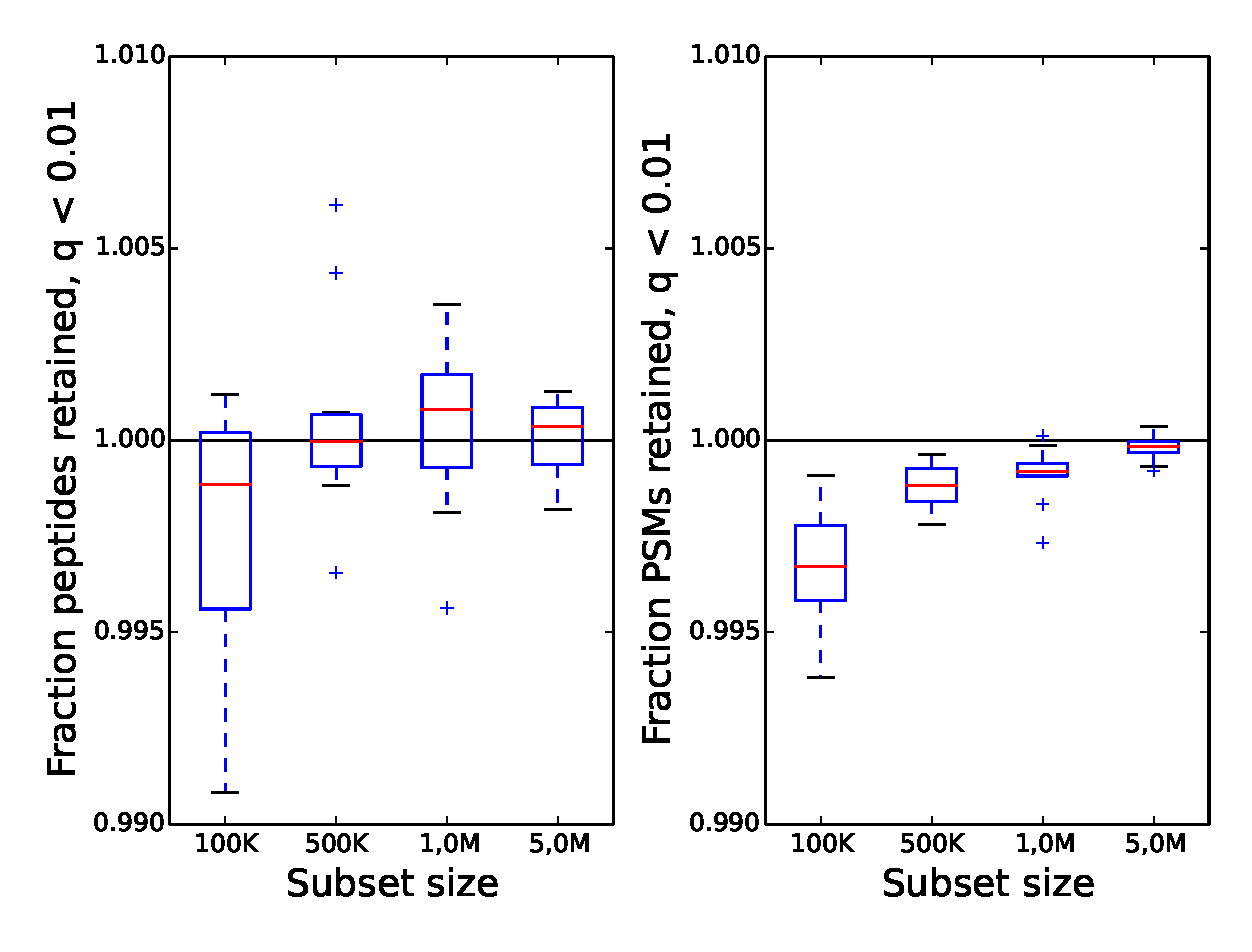
\includegraphics[width=0.6\linewidth]{./img/subset-performance}
\caption{\label{fig:subset}\textbf{SVM training on downsampled data
    retains the performance achieved using the full data set.}  From
  the full Kim data set of $73$ million target+decoy PSMs, we
  evaluated subset sizes of $100\,000, 500\,000, 1\,000\,000$ and
  $5\,000\,000$ PSMs to train the SVMs, repeating this for $10$
  randomized sets, and scored all $73$ million PSMs using the
  resulting support vectors. The figure plots the ratio of significant PSMs
  and peptides at a $q$ value threshold of $0.01$ as the fraction
  compared to using the full training set of $73$ million PSMs. The
  number of significant PSMs and unique peptides does not drop
  significantly, even for subsets of $100\,000$ PSMs.}
\end{center}
\end{figure}

We used the Kim data set to evaluate the robustness of Percolator's
SVM classifier to reductions in the size of the training set.  The
Tide searches of the complete Kim data set against the human Swissprot
database resulted in $73$ million target and decoy PSMs.
Post-processing the full data set with Percolator resulted in
$7\,928\,454$ significant PSMs and $298\,301$ unique target peptides
at a $q$~value threshold of $0.01$.  To characterize the performance
of the SVM learning procedure when training on subsets of the PSMs, we
randomly selected subsets of $100\,000, 500\,000, 1\,000\,000$ and
$5\,000\,000$ PSMs from the Kim set.  We trained using these subsets
and applied the trained classifier to the full data set. Preliminary
results showed that including target and decoy PSMs belonging to the
same spectrum together during the selection of random subsets gave a
more stable performance than sampling without taking this into
account. Therefore, this strategy was applied in the random sampling
process. For each random subset size, we calculated the mean and
standard deviation over $10$ randomized runs of the number of PSMs and
peptides with $q$ value below $0.01$.

This experiment showed that using subsets as small as $100\,000$ PSMs
($0.14\%$) for SVM training did not significantly reduce the number of
identified peptides and PSMs (Figure \ref{fig:subset}). The standard
deviation of identified PSMs across the randomized runs for a fixed
subset size did seem to increase slightly when taking increasingly
smaller subsets, but this effect was limited. By using a subset of
$500\,000$ PSMs to train the SVM, Percolator's runtime was reduced
from almost a full day to less than $10$ minutes. Furthermore, the
memory consumption dropped from almost $100$~GB to just $10$~GB,
allowing analysis of this type of large-scale data to be done on
commodity computers.

\subsection*{Protein-level FDR estimates are poorly calibrated when
  shared peptides are retained}

\begin{figure}
\begin{center}
\begin{tabular}{ccc} 
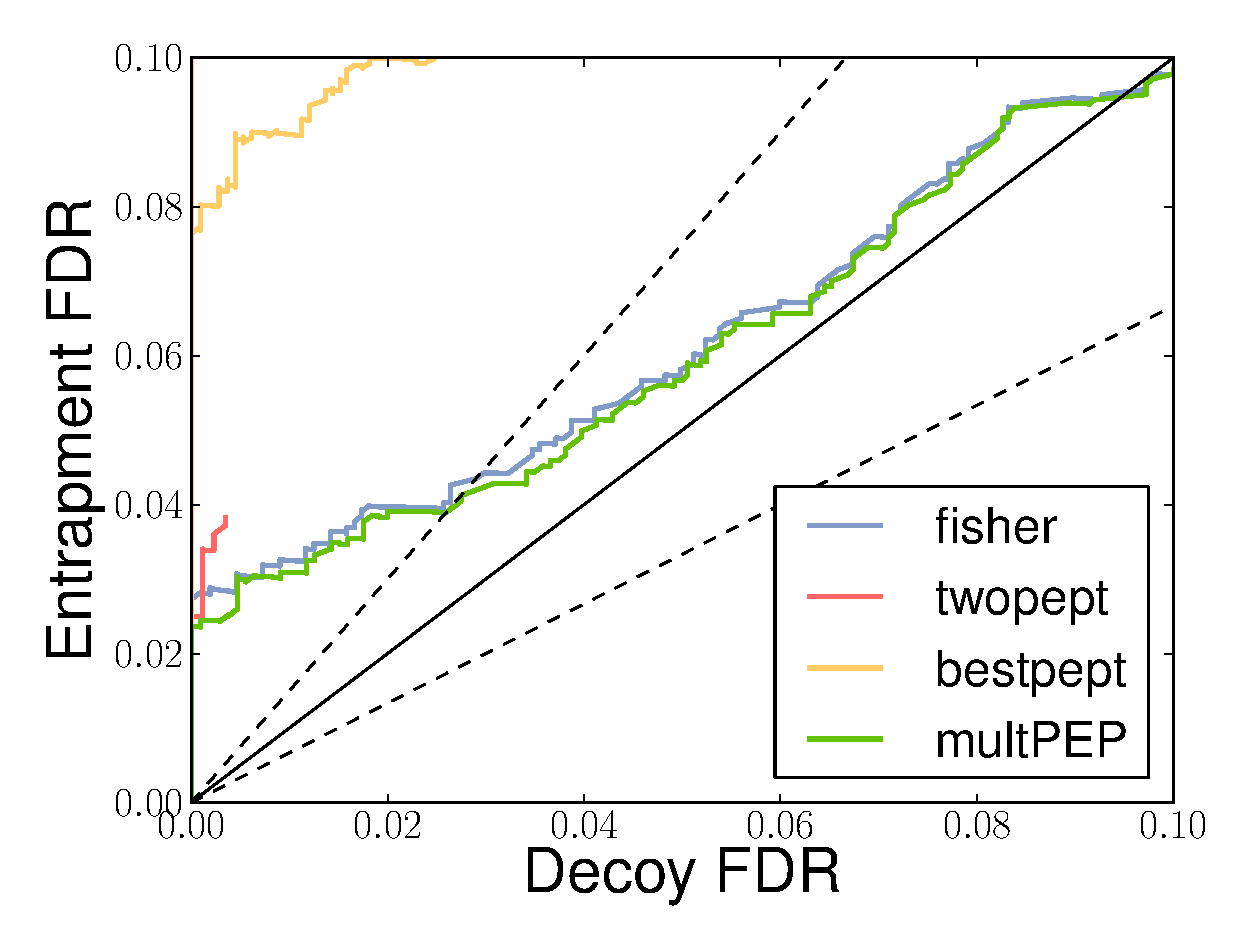
\includegraphics[width=0.3\linewidth]
  {./img/shared-pept-accuracy-fdr10} &
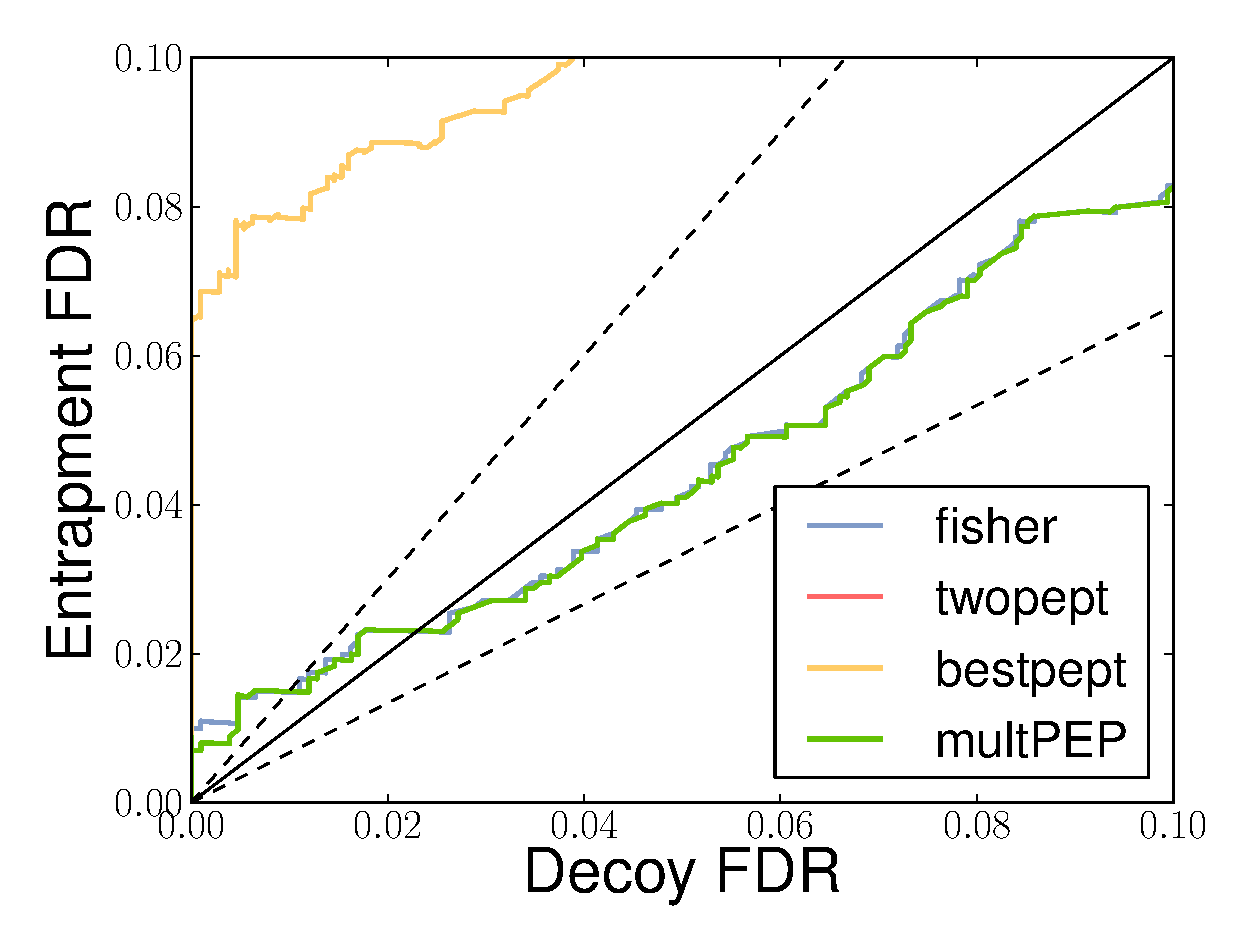
\includegraphics[width=0.3\linewidth]
  {./img/shared-pept-accuracy-fdr5} & 
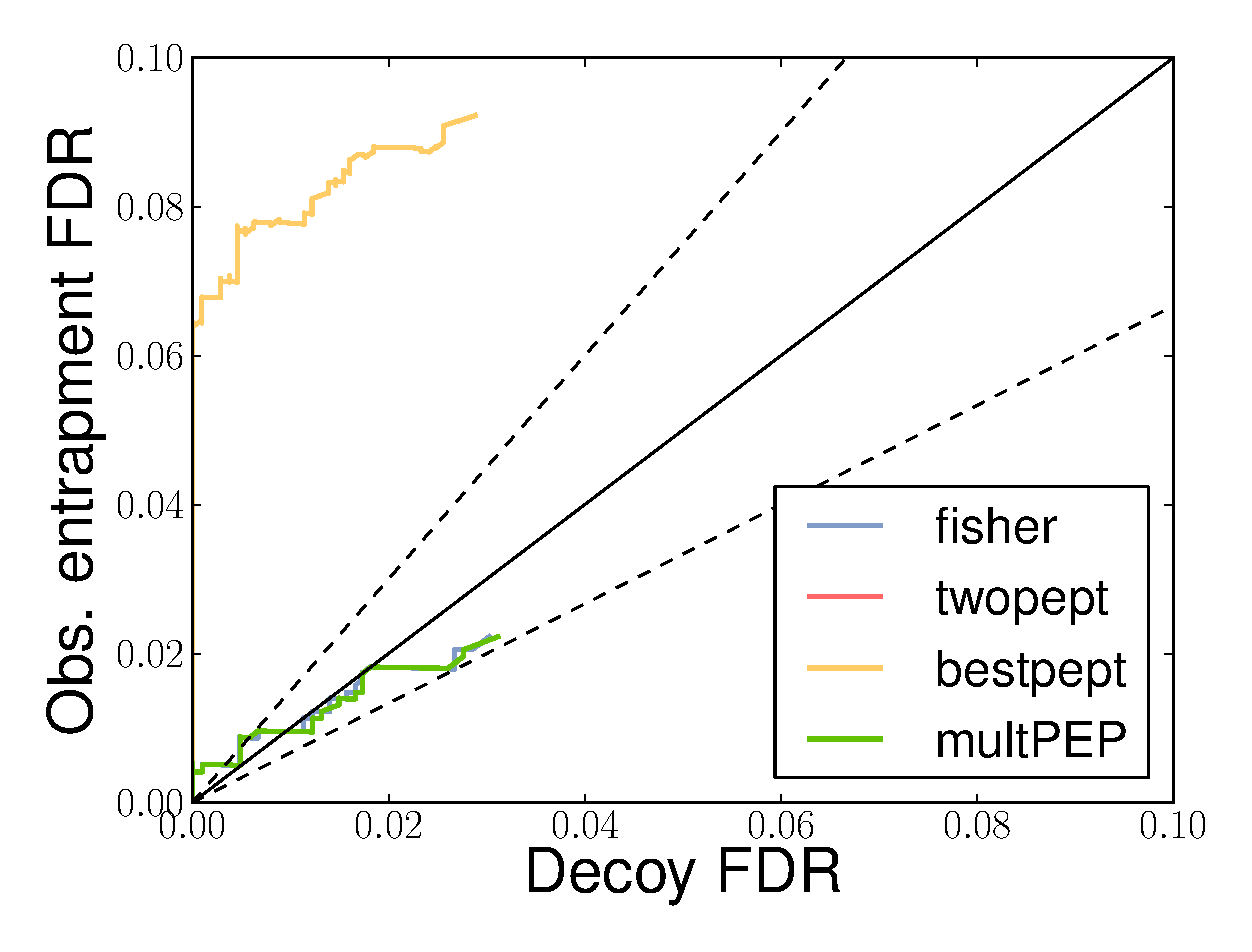
\includegraphics[width=0.3\linewidth]
  {./img/shared-pept-accuracy-fdr1}\\
(A) & (B) & (C)
\end{tabular}
\caption{\label{fig:shared-accuracy}\textbf{Retaining shared peptides
    leads to poor calibration of the decoy model for all protein
    inference methods.} The figures plots reported $q$~values from the
  decoy model, the decoy FDR, against the fraction of entrapment
  proteins in the set of identified target proteins, the observed
  entrapment FDR using a peptide-level FDR threshold of $10\%$ (A),
  $5\%$ (B) and $1\%$ (C). Dotted lines correspond to $y=1.5x$ and
  $y=0.67x$.  For a peptide-level FDR threshold of $10\%$, all four
  methods produce anti-conservative FDR estimates, with Fisher's
  method and product of PEPs achieving reasonable accuracy above $3\%$
  decoy FDR. For the stricter thresholds of $5\%$ and $1\%$ the FDR
  estimates of those two methods are anti-convervative for very low
  FDRs, but quickly become conservative for higher FDRs.}
\end{center}
\end{figure}

We assessed the accuracy of decoy-based FDR estimates derived using
four protein inference methods---best-scoring peptide, two-peptide
rule, product of PEPs, and Fisher's method---by analyzing the
hm\_yeast set.  The assessment employed our previously described
sample/entrapment strategy \cite{granholm2013determining}, which
involves comparing the $q$~values reported based on the decoy model,
the decoy FDR, to the fraction of entrapment proteins in the set of
identified target proteins, which we call the observed entrapment FDR.

First, we compared the four protein inference methods while retaining
shared peptides. We grouped proteins that had the same set of
identified peptides, and also added proteins whose identified peptides
formed a strict subset of this set to each
group~\cite{serang2012review}.  {\em FIXME: find a better reference
  for protein grouping approach? --Matthew} To reduce the effect of
proteins breaking away from the group due to low-scoring, incorrect
peptide identifications that are unique to that protein, a
peptide-level FDR threshold was set at $10\%$.

This experiment showed that the decoy models based on the reversed
protein database systematically produce liberal (anti-conservative)
FDR estimates (Figure \ref{fig:shared-accuracy}). Fisher's method and
the product of peptide-level PEPs are most liberal for small
thresholds but manage to provide better estimates above $\sim 3\%$ and
$\sim 1\%$ protein-level FDR for $10\%$ and $5\%$ peptide-level FDR
thresholds, respectively. For the two-peptide rule, not enough decoy
proteins remain to see if the FDR estimates will become more accurate
at some point, and the best-scoring peptide approach produces
dramatically liberal estimates for all thresholds. Taking stricter
peptide-level thresholds generally improved the accuracy for Fisher's
method and the product of PEPs. Going down to $5\%$ peptide-level FDR
still produced anti-conservative protein-level FDR estimates in the
region below $1\%$ protein-level FDR, but going further down to $1\%$
peptide-level FDR actually produced reasonable, though still slightly
anti-convervative, estimates in that region.

\subsection*{Eliminating shared peptides improves calibration}

\begin{table}
\caption{\label{tab:duplicate-proteins}\textbf{Protein grouping
    increases the number of identifiable protein entities.}}
\scriptsize
\begin{center}
\begin{tabular}{lrrr}
\hline
& Swissprot & Swissprot+TrEMBL & Ensembl\\
\hline
Protein sequences & 20\,201 & 69\,714 & 101\,933\\
Peptide sequences & 586\,424 & 664\,801 & 672\,519\\
Proteins with protein-specific peptides & 19\,938 & 52\,834 &
49\,871\\
Protein groups & 20\,104 & 58\,605 & 68\,370\\
Protein groups with protein group-specific peptides & 19\,978 &
54\,292 & 58\,929\\
\hline
\end{tabular}
\end{center}
\end{table}

We hypothesized that these calibration problems arise from the
peptides that are shared between different proteins in the database.
Accordingly, we next considered an approach that discards shared
peptides, retaining only those that are unique to a single protein.
To reduce the effect of ``fictitous'' shared peptides that correspond
to protein fragments or other truncated protein forms, we used the
approach to handling shared peptides from Nesvizhskii {\em et
  al.}~\cite{nesvizhskii2003statistical}. Here, proteins are mapped to
their theoretical proteolytically digested peptides, rather than their
experimentally discovered peptides, and two proteins $A$ and $B$ are
merged into a group if protein $A$'s peptides are a superset of
protein $B$'s peptides or vice versa.  We then retain the peptides
that are unique to a protein group, rather than to a single protein.

We applied this approach to several protein databases and showed
empirically that including the protein grouping step increases the
number of protein entities, {\em i.e.}, single proteins or protein
groups, with a peptide uniquely identifying it.  The experiment
involved performing a fully tryptic digestion, with no misssed
cleavages, of three human protein databases---Swissprot,
Swissprot+TrEMBL, and Ensembl---considering peptides with lengthsk of
6--50 amino acids. TrEMBL and Ensembl contain many proteoforms and
therefore benefit significantly from this particular protein grouping
approach in terms of number of identifiable protein entities (Table
\ref{tab:duplicate-proteins}). Note that, unfortunately, some protein
groups will remain unidentifiable, because all their peptides are
shared with at least two different protein groups.

\begin{figure}
\begin{center}
\begin{tabular}{cc} 
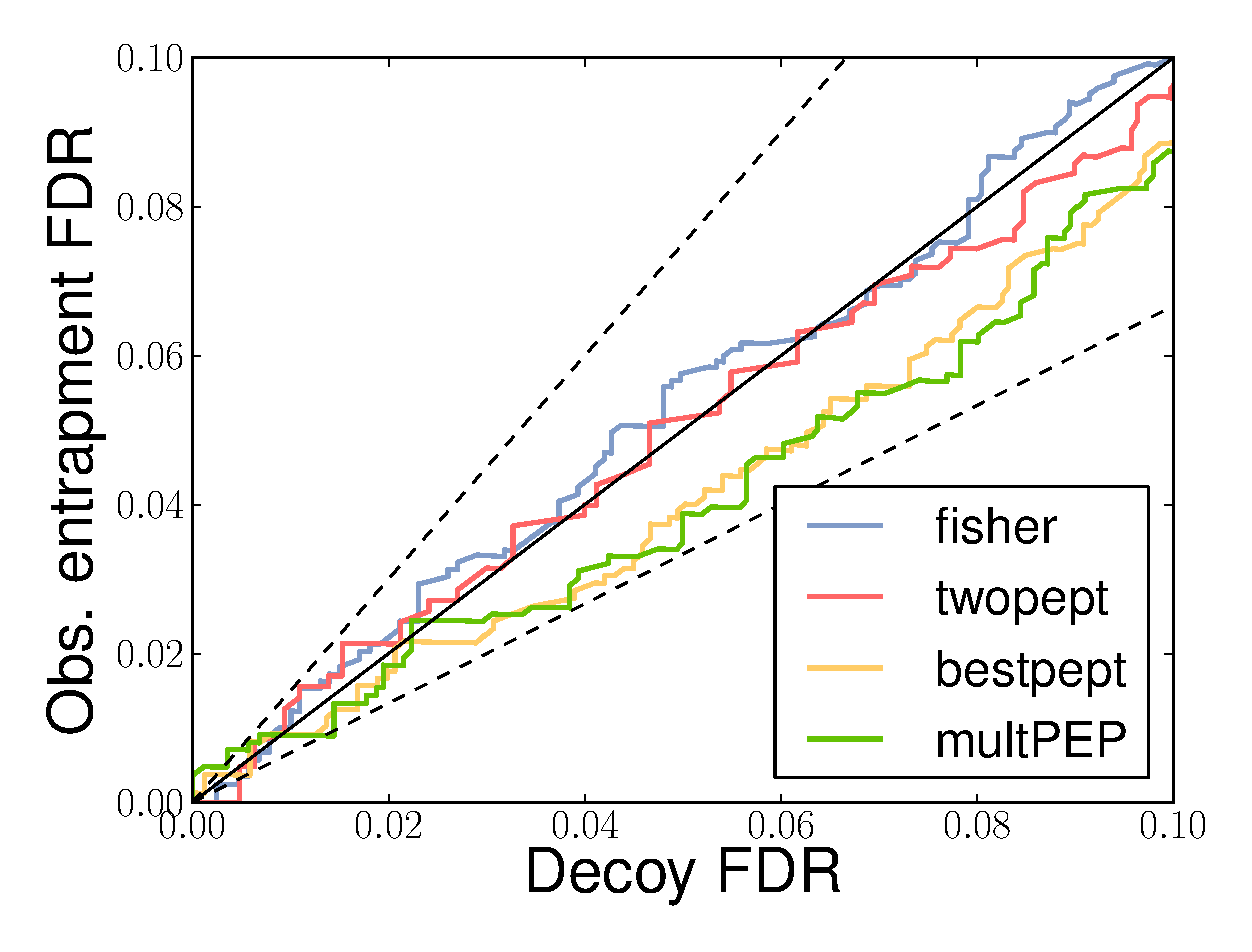
\includegraphics[width=0.45\linewidth]{./img/unique-pept-accuracy} &
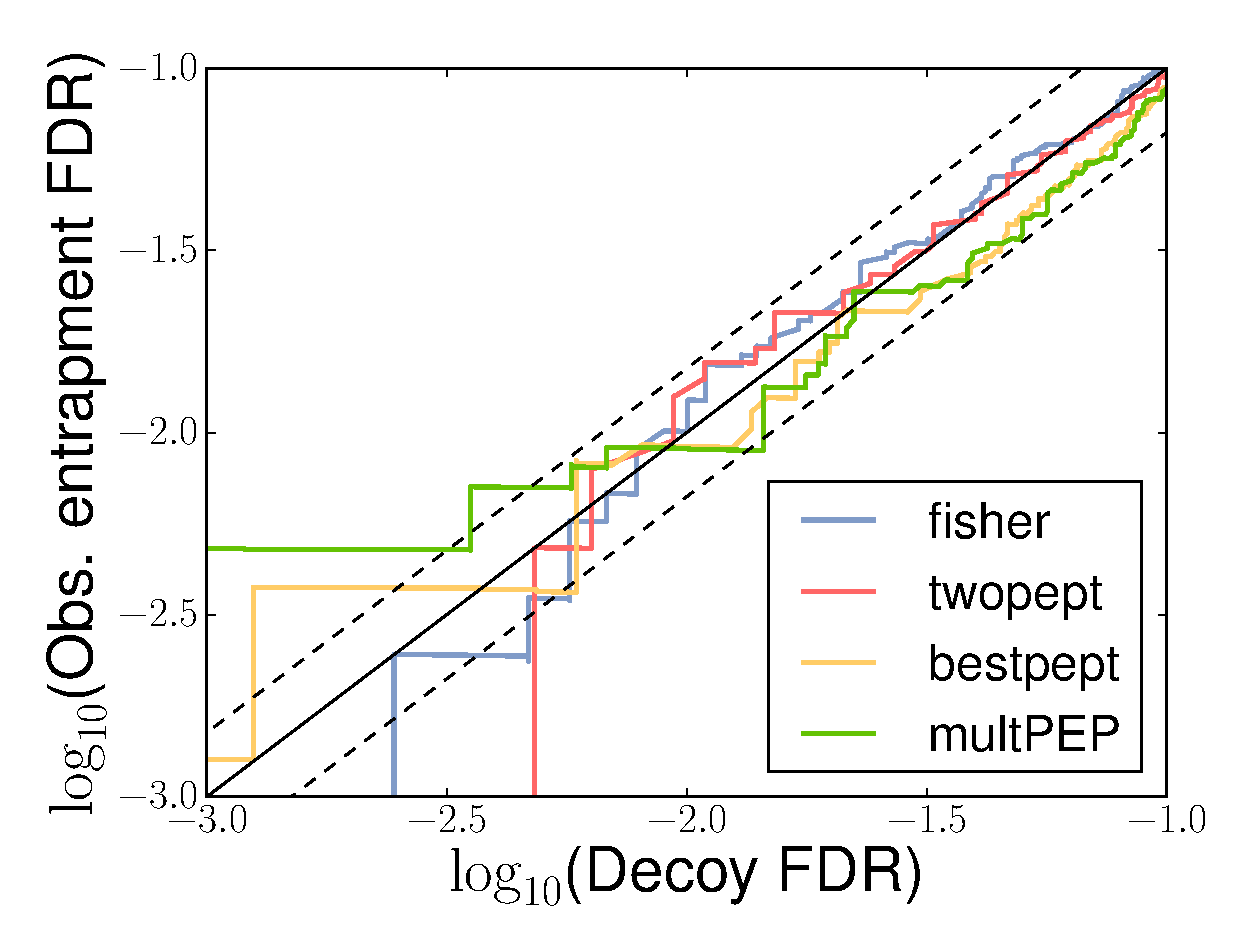
\includegraphics[width=0.45\linewidth]{./img/unique-pept-accuracy-log}\\
(A) & (B)
\end{tabular}
\caption{\label{fig:unique-accuracy}\textbf{Using only protein-unique
    peptides gives accurate estimates of the protein-level FDR.}
  (A) The figure plots the decoy FDR against observed entrapment FDR. 
  All four methods produce accurate FDR estimates. (B) A logarithmic 
  plot of the region $[0.001, 0.1]$ with the same axes as in (A).}
\end{center}
\end{figure}

Having eliminated the shared peptides, we returned to our
sample/entrapment strategy for estimating the accuracy of
protein-level FDR estimates.  In this new setting, all four methods
now gave accurate protein-level FDR estimates (Figure
\ref{fig:unique-accuracy}A).  Zooming in on the low FDR region (Figure
\ref{fig:unique-accuracy}B) showed that the protein-level FDR
estimates break down somewhere in the $[0.001, 0.01]$ range,
presumably due to the low density of decoy proteins in that region.
From these results, it became clear that taking only unique peptides,
together with the protein grouping approach from Nesvizhskii {\em et
  al.}, would be the most robust choice, regardless of the protein
inference method.

\subsection*{Selection of a protein inference strategy}

\begin{figure}
\begin{center}
\begin{tabular}{ccc} 
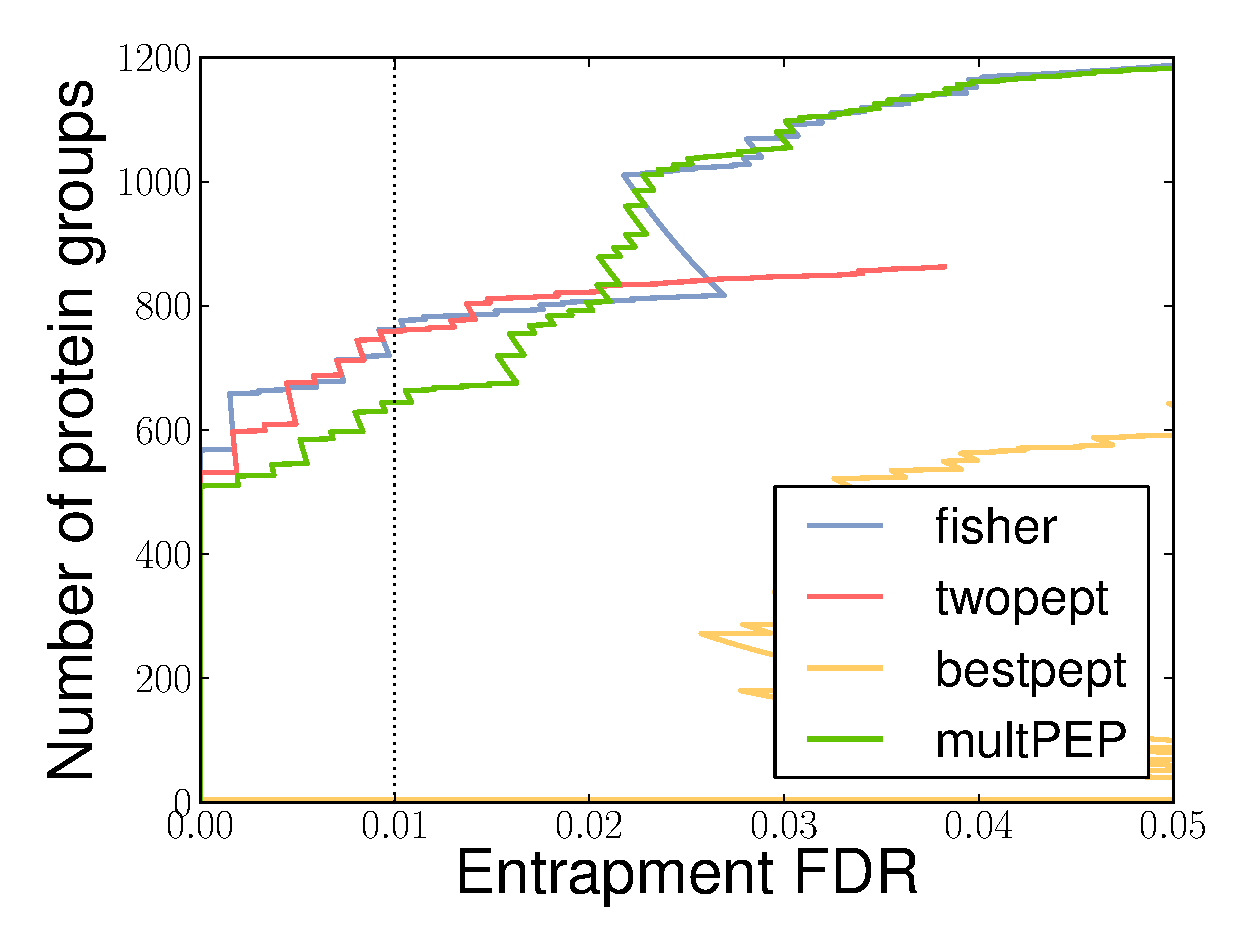
\includegraphics[width=0.3\linewidth]
  {./img/shared-pept-performance-fdr10} &
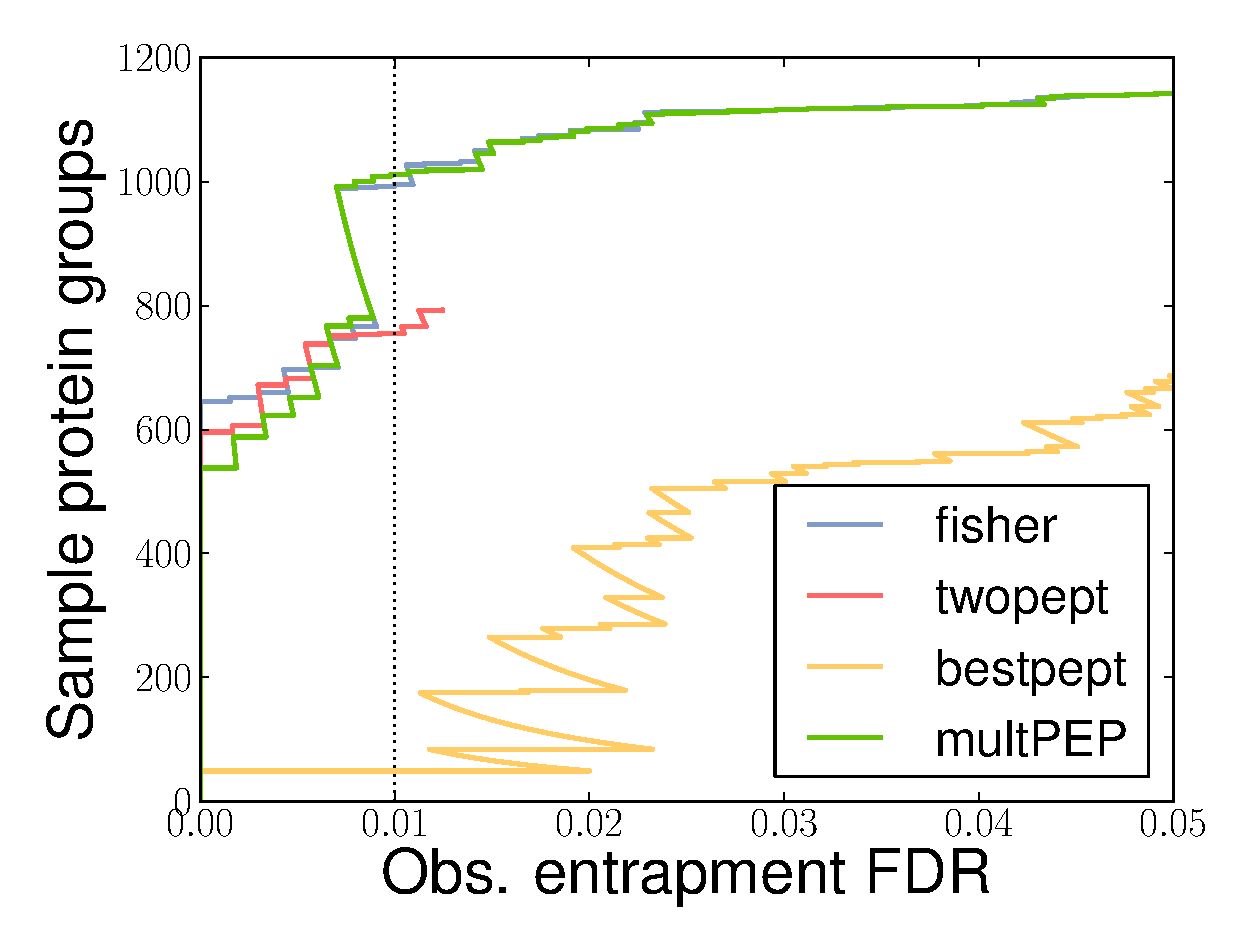
\includegraphics[width=0.3\linewidth]
  {./img/shared-pept-performance-fdr5} &
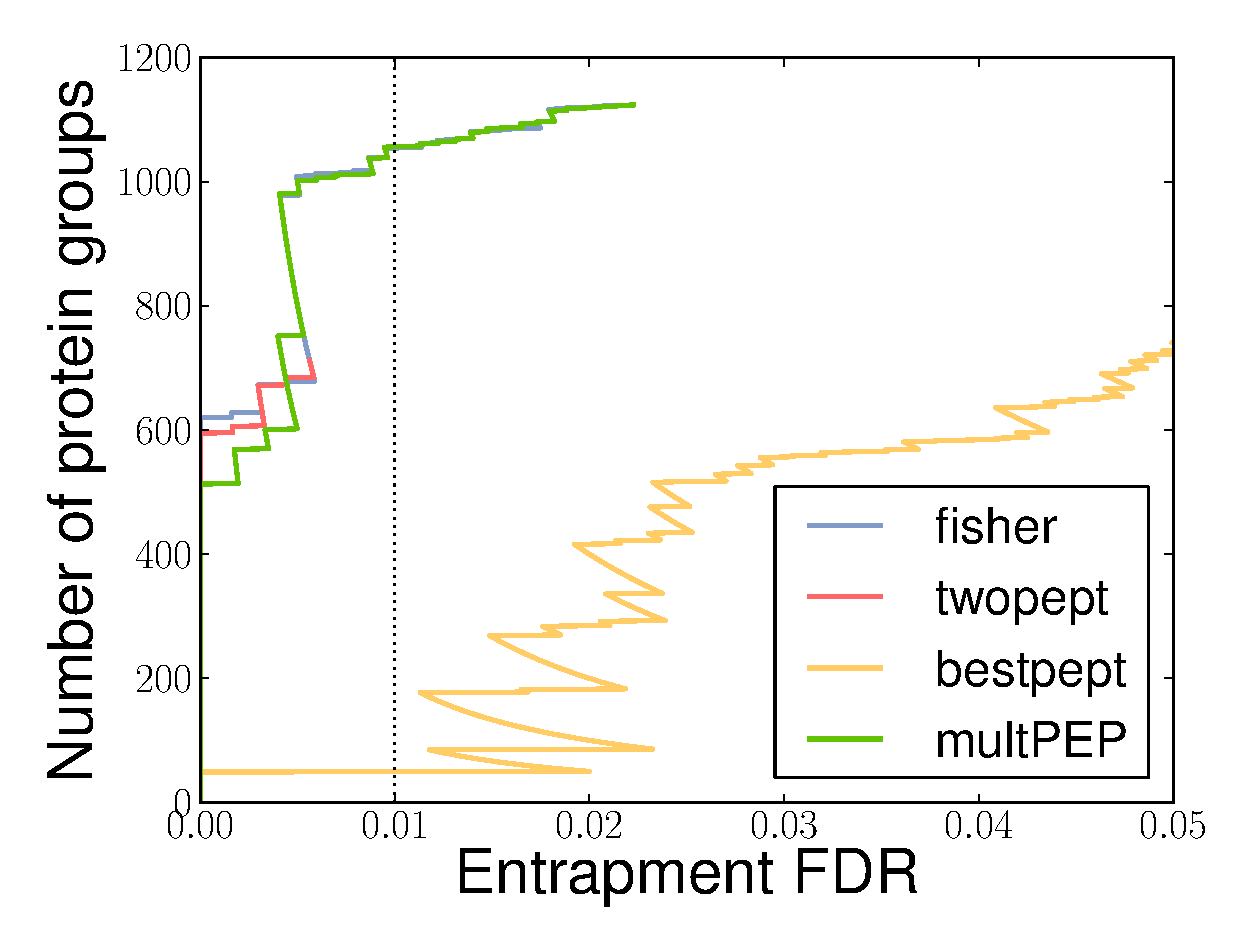
\includegraphics[width=0.3\linewidth]
  {./img/shared-pept-performance-fdr1}\\
(A) & (B) & (C)
\end{tabular}
\caption{\label{fig:shared-performance}\textbf{Comparison of protein 
detection methods when retaining shared peptides.} We plotted the 
number of sample proteins, which can be considered an estimate for the 
number of true identifications, against the observed entrapment FDR 
using a peptide-level FDR threshold of $10\%$ (A), $5\%$ (B) and $1\%$ 
(C). Whereas Fisher's method, the product of peptide-level PEPs and 
the two peptide rule initially pick up many sample proteins, the best 
scoring peptide approach immediately breaks down. Stricter 
peptide-level thresholds increase the number of protein detections at 
$1\%$ protein-level FDR for the $3$ other methods. {\em FIXME: The 
text never specifically refers to panel B.  Perhaps it should be 
deleted.  --Bill. I think it is a useful plot to have, as some readers 
might wonder if the decreased accuracy is worth it if the performance 
is much better. I moved it to the ``Selection of a protein inference 
strategy'' section. --Matthew}}
\end{center}
\end{figure}

{\em FIXME: Need some text to accompany the figure with performance 
of retaining shared peptides. An important point to make is that the 
protein groups contain on average 3 to 4 proteins, opposed to an 
average of 1.02 when only using unique peptides. --Matthew}

\begin{figure}
  \centering
  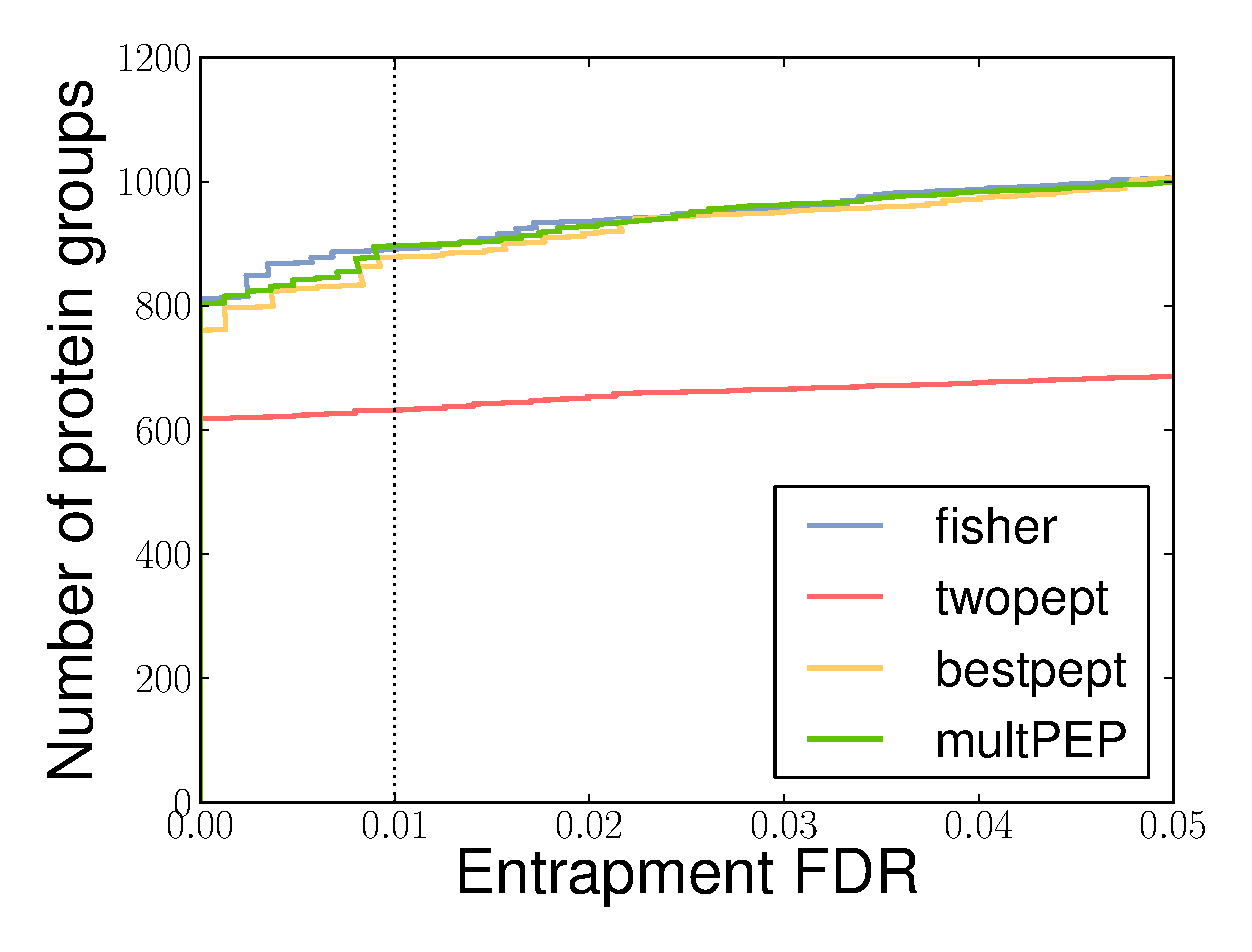
\includegraphics[width=0.45\linewidth]{./img/unique-pept-performance}
  \caption{{\bf Comparison of protein detection methods.}  The figure
    plots the number of accepted protein groups against the observed
    entrapment FDR for (A) the hm\_yeast and (B,C) Kim data
    sets. Fisher's method, the product of peptide-level PEPs and the
    best scoring peptide approach all perform about equally, while the
    two peptide rule is much less sensitive.  {\em FIXME: Isn't it
      worrisome that, for the yeast data set, the best-scoring peptide
      approach seems to do worse than Fisher and multPEP? --Bill. 
      Yes it is, but I guess we are mostly interested in the 
      performance on large-scale data sets in this paper. --Matthew} 
      {\em FIXME: What about adding two more panels for the Kim data 
      set and getting rid of the table?  --Bill. Sounds good, I 
      don't have time to produce them now but I will add them next 
      time. --Matthew}}
  \label{fig:power}
\end{figure}

Finally, we compared the number of proteins detected as a function of
the observed entrapment FDR for the different inference methods.  For
the hm\_yeast data set, the two-peptide rule was the only method
clearly performing worse than the others (Figure~\ref{fig:power}A).
We then repeated the assessment on the much larger Kim data set, using
two different databases (Swissprot and Swissprot+TREMBL).  Even for
such large-scale data, all four protein inference methods took less
than a minute of processing time due to their simplicity. We looked at
the number of identified proteins at $1\%$ reported protein-level FDR
(Table~\ref{tab:pandey-stats}).  The best scoring peptide approach
identified the most protein groups with a $3\%$ margin over the second
best method. Fisher's method identified much fewer proteins than the
other three methods, due to incorrect peptides dragging down the $p$
value of correct proteins. {\em FIXME: The previous sentence is an
  interesting observation. I think you should do some kind of
  follow-up analysis to verify this hypothesis. --Bill. I have 
data for the Kim set using a fully tryptic search. This significantly 
improved the performance of Fisher's method, most likely because less 
spurious peptides were present per protein. I don't know if that 
qualifies as a follow-up analysis, but it might be interesting to show
anyway. --Matthew} Although the
many proteoforms in the TrEMBL database caused a large drop in the
number of identifications for all methods, the relative ranking of
methods was consistent in both sets of results. Overall, we concluded,
in agreement with Savitski {\em et al.} \cite{savitski2015scalable},
that the best-scoring peptide approach yielded the best overall
performance.  We therefore implemented this protein inference method
in the latest Percolator package.

\begin{table}
  \begin{center}
    \begin{tabular}{lrr}
    \hline
    partial digestion & Swissprot & Swissprot+TrEMBL\\
    \hline
    Best scoring peptide & 12\,370 & 5\,909\\
    Product peptide-level PEPs & 11\,968 & 5\,626\\
    Two peptide rule & 11\,409 & 4\,231\\
    Fisher's method & 8\,964 & 3\,717\\
    \hline
    \end{tabular}
  \end{center}
\caption{\label{tab:pandey-stats}\textbf{Using the best-scoring
    peptide as a protein's representative identified the most protein
    groups.} We examined the number of protein identifications for the
  four protein inference method using only peptides unique to one of
  the protein groups formed by the approach from Nesvizhskii {\em et
    al.}. }
\end{table}

\section*{Discussion}

We demonstrated that Percolator 3.0 can calculate protein-level FDRs
on a human proteome scale study, in this case $73$ million PSMs, in a
matter of minutes on a commodity computer.

The subset scoring shows great stability even when only sampling a
tiny fraction, as small as $0.1\%$, of the original number of PSMs.
The {\em Kim} set might not be as representative for other types of
studies that have greater heterogeneity, but it seems likely that the
idea will hold as long as the subsets are not chosen too small.
Particularly our subset sampling strategy, that trains and tests on
the same data will only avoid problems of overfitting when the
strategy is carried out on large datasets.

The most successful protein inference method turned out to be the one
where proteins were grouped by their theoretical peptide sets and only
the best scoring peptide was considered. This implies that the
algorithm excludes the majority of the PSMs in its final protein list,
something that may feel quite unsatisfying. With regards to the
discarded shared peptides, large-scale studies give us the luxury of a
deep coverage of the present peptides and therefore identify many
peptides that are unique to a protein. This mitigates the problem of
ignoring shared peptides in terms of number of protein identifications
and makes the task of protein inference much simpler and intuitive.

The main problem in including the evidence of the other lower scoring
peptide identifications is the difficulty in dealing with incorrect
peptide identifications belonging to correct protein identifications.
This can clearly be seen in the poor performance of Fisher's method
for combining $p$ values on the {\em Kim} set. Setting
peptide-level thresholds can actually bring Fisher's method up to par
with the best scoring peptide approach (data not shown). However,
it does not produce significantly more protein identifications,
while introducing an extra parameter that needs to be set correctly.

The protein grouping of Nesvizhskii {\em et al.} employed here still
suffers from the problem that an identification of a protein group
leaves open the question which proteins in the group are actually
correct. Here, we interpreted it using the null hypothesis that all
proteins in the group are incorrect, {\em i.e.}, an identified protein
group means that we expect at least one of the proteins to be correct,
but we are agnostic about which one. Compared to the conventional
protein grouping approach, however, the groups are much smaller and
this unsatisfactory answer does not have to be given as often.
Furthermore, if genes, rather than proteoforms are the entities of
interest, using databases with few proteoforms such as Swissprot
should do the job.

The construction of the entrapment database should be considered as a 
rather crude approximation of true experimental settings and could be 
improved upon in future work. While it does conserve homologs by 
shuffling peptide rather than protein sequences, it only allows for 
simulation of fully-tryptic peptides without miscleavages. 
Furthermore, the mechanism that creates shared peptides between sample 
and entrapment database does not do any attempts to model homology. 
The shared peptides are randomly distributed over all proteins, while 
in practice we can expect some portion of proteins sharing multiple 
peptides and many proteins having no shared peptides at all. The rate 
of shared peptides of $4\%$, modelled after the Swissprot yeast 
database, is also a good approximation of the shared peptide rate of 
the Swissprot human database. However, the shared peptide rate in the 
Swissprot+TrEMBL database is much higher with over $60\%$ of the 
peptides being shared by at least two proteins, which could result in 
significantly different outcomes.

We realize that other parts of the shotgun proteomics analysis
pipeline might still have significantly higher computing requirements
than Percolator, but fortunately these can often readily be
parallelized as the runs can be analyzed independently. However,
obtaining significance measures per run or data set and combining them
afterwards is not at all straightforward and should be handled with
the greatest caution~\cite{serang2015solution}. This new version of
Percolator opens up for the possibility of easily obtaining
statistical significance measures on aggregated data from a great
number of runs without running this risk.

\section*{Acknowledgements}

This work was supported by National Institutes of Health award P41~GM103533.

%FIXME: add acknowledgement to Uppmax? LK: Check standard formulation
% from SNIC

\bibliographystyle{plain}
\bibliography{percolator}

\end{document}
